%\chapter{Background}
In this chapter we will provide some background needed for this thesis.

\section{Distributed Systems}\label{background:distributed_systems}
In the start of their book, Steen and Tanenbaum\cite{steen_distributed_2017} defines distributed systems loosely: 
\say{A distributed system is a collection of autonomous computing elements that appears to its users as a single coherent system.}

This definition describes two important characteristics of distributed systems. Firstly, we can think of a distributed system as several computers or programs that work independently. They share workload and storage between, but they are independent in the same sense as processes. The different programs or computers are referred to as Nodes. Each node in the system will work concurrently. This is one of the great benefits of a distributed system. This is because you can share heavy computational tasks across the system to make it distribute the load. A computer can have several nodes, but usually we think of different computers as different nodes. The other characteristic it describes, is that the users should only see a single coherent system. That means that the user should not notice that the application is running on a distributed system, unlike an application running on a single computer.

Distributed systems have no shared clock. This is because having a shared clock is almost impossible, as even atomic clocks is not accurate enough and other factors will affect the clocks. Therefore, you have to utilize other methods to ensure synchronization. We will discuss synchronization in section \ref{cascading_search}. Each node will therefore have an independent notion of time, and the system as a whole will not have a global clock\cite{steen_distributed_2017}. This is also important because even though the nodes work with each other, they should always be loosely coupled and as independent as possible.

The nodes will exchange information, but they don’t have shared memory. This is to ensure \textit{loose coupling}, which means that nodes are not too dependent on each other. In some systems it is also important with loose coupling because the nodes in the system can be heterogeneous. Two nodes can have quite different environments, such as different OS, processing power, network, memory and hardware, but still work together in a distributed system. Having a loosely coupled system will ensure that the system is robust and that you don't need specific hardware to run it, but can rather focus on the other layers. 

A distributed system is dynamic, which means that nodes may leave or join the system at any time. This is useful for scaling, as one can easily add nodes after demand. However, it also raises the issue that a node might disappear while doing a task, which is important to handle.



\subsection{Distribution Transparency}
To make a distributed system seem like one system, is called Distribution Transparency. You don't want the user to know that it is interacting with a distributed system. Steen and Tanenbaum brings up several types of transparency that helps achieve distribution transparency. Here is a brief description of them.

\subsubsection{Access Transparency}
Access Transparency is about hiding differences in machine architectures. The nodes need to agree on how to represent data. This helps the application use local and remote resources as the same. 

\subsubsection{Location Transparency}
Location Transparency is about not letting the user tell where an object is physically located in the system. It should seemingly be local, but might be on a different computer.

\subsubsection{Relocation Transparency}
Relocation Transparency is about hiding when an object is moved from one node to another while it is in use. The application should still be usable and the user should not notice that the object has moved.

\subsubsection{Migration Transparency}
Migration Transparency is about offering the mobility of resources to the users. The users can in other words change the location of objects, without it disrupting the program. In other words relocation transparency is about being moved, while migration transparency is about letting the users move the objects.

\subsubsection{Replication Transparency}
Replication transparency is about hiding when an object is replicated. It can be hard to keep all replicas up to date, but the users should not know which replica it is accessing.

\subsubsection{Concurrency Transparency}
Concurrency Transparency is about not letting users know that they are accessing the same objects at the same time. For example, if several users are accessing the same database, they should not notice that other users are also querying the same database.

\subsubsection{Failure Transparency}
Failure Transparency is about hiding a object or node failure from a user. One should not assume that a node will  never crash or become unreachable. The system should be able to recover and handle fails without the user noticing.


\subsection{Advantages}
Some of the advantages of distributed systems are scalability, reliability, fault tolerance and increased performance. Each of the characteristics is on its own very good to have, but the sum of them is what makes distributed systems incredibly good.

\subsubsection{Scalability}
Scalability is about being able to scale up to meet demand. As more and more computation and storage move to the cloud, this is very important. Scalability can be measures in three different dimensions, namely \textbf{Size, Geographical and Administrative scalability}.

\textbf{Size scalability} is about being able to add more resources and clients to the system without loss of performance \cite{steen_distributed_2017}. Scaling is challenging as there is many factors that can act as a bottleneck. For instance, it does not matter how big you data centre is, if the bandwidth  is too small to handle all the users. Another example is that the hardware might not be fast enough. To ensure that the system is able to handle a continuously increasing amount of users and requests, you have to handle these kind of bottlenecks. Most of the problems does come from lack of resources on the servers. To fix this you can upgrade the hardware, which is referred to as scaling up, or deploy more servers, which is referred to as scaling out.

\textbf{Geographical Scalability} is about having nodes (most likely servers) that are far from the client, but the delay from communicating with them is hardly noticed. In a wide-area system, we might have nodes on different continents. The delay of sending messages between them is then too high to not be noticed in some situation. Also, because the packets are traveling through so many switches and routers, it is much less reliable. Some stretches might also have limited bandwidth, which might be a bottleneck for the system. You also cant just put a distributed system designed for a local-area network(LAN) on a wide-area network(WAN). For example, if your system relies on broadcasting. Broadcasting will work fine on a LAN but will probably work pretty terrible on a WAN. To mitigate latency issues, you can try to minimize waiting for a result. You do this by using asynchronous communication, which means that you avoid waiting for a result from others as much as possible. In applications where this is not possible, for example with Augmented Reality, we have to either reduce the amount of communication or move the server closer to the client.

\textbf{Administrative Scalability} is about scaling a distributed system across several independent administrative domains \cite{steen_distributed_2017}. This can be hard, as the domains can use different rules and conventions for communication, payment, resource usage, read-write privileges and etc. There is also a security aspect of it, as the domains might have different views on security, that might be conflicting. 



\subsubsection{Fault Tolerance}
A distributed system should be fault tolerant. When something fail, for example if a node goes down, then the system should be able to handle it with out the user or client knowing. This is one key characteristic of distributed systems, since it is often spread over several nodes, we can easily avoid having a single point of failure. Therefore it is called a \textit{partial failure}\cite{steen_distributed_2017} when something fails in a distributed system. 
Fault tolerance is really important to help keeping the system reliable and maintainable. 

\subsubsection{Performance}
There is little reason to use distributed systems if you do not get a performance boost while using it. Of course there are other reasons, like fault tolerance or convenience, but performance is at the heart of distributed systems. The fact that you can distribute the workload across several machines will in most cases give you a significant speed-up. Having several machines able to receive requests lets you have tremendous pressure from millions of requests without problems.
To split the workload we need multiprocessing. Multiprocessing lets us divide different work do different machines. For example, it can be one machines job to receive requests and forward them to a set of machines who do the actual work. Essentially it enables doing things in parallel, which is what gives us speed-up in first place.

\subsection{Pitfalls}
Steen and Tanenbaum \cite{steen_distributed_2017} brings up several pitfalls that you should avoid when making a distributed system:
\begin{itemize}
    \item The network is reliable
    \item The network is secure
    \item The network is homogeneous
    \item The topology does not change
    \item Latency is zero
    \item Bandwidth is infinite
    \item Transport cost is zero
    \item There is one administrator
\end{itemize}
All of these are important to have in mind while creating a distributed system. However we will mostly focus on \textbf{The network is homogeneous, The topology does not change, Latency is zero, Bandwidth is infinite} in this thesis. 

\textbf{The network is homogeneous}
In IoT we are dealing with a very heterogeneous network. Most of the devices do not use the same architecture or hardware.

\textbf{The topology does not change}
This is not true at all in the era of IoT. There is tons of mobile devices, like cellphones, that move around all the time, and changes the topology of the network. When going any further out than a LAN, we are also using hardware that we do not have control over. This means that they can move or disappear at any time.

\textbf{Latency is zero}
In a wide-area distributed system, the latency can be quite high. If you assume the latency is zero, then we can run into problems that will affect the client quite a bit. Since the results can take some time to come back we get a lot of waiting time, that is not taken into account. The user is then affected by this, as it has to wait for the client. 

\textbf{Bandwidth is infinite}
When you have a case where you need to use a lot of bandwidth to use the application, it is important to have enough bandwidth. If you need to send more data than one part of the link between the nodes can handle, then you will probably get a substantial loss of quality on the client. 


\subsection{Middleware}
To ease the development process in distributed systems we need middleware. Middleware is a layer running on top of the OS of each machine in the system, and connects all the applications running on top of it. It provides and interface to the application, which helps the application with resource management, communication with other nodes, security and recovery\cite{steen_distributed_2017}. An example of a middlware is the Emerald VM, which we will discuss in the Emerald section \ref{Emerald}. 


\subsection{Types of Distributed systems}
% on example of a cluster computing system is PlanetLab, which we will talk about later.
Distributed systems can generally be divided into two types: \textbf{Cluster computing and Grid computing}.

\subsubsection{Cluster computing}
Cluster computing is a collection of computers that usually has homogeneous architecture and hardware, as well as being in about the same place geographically. These computers usually run the same OS and are used to effectively distribute (and therefore parallelize) heavy computational tasks. They are able to easily communicate because of the small latency and high reliability of LAN's. Data centres are an example of Cluster computing. 

\subsubsection{Grid computing}
Grid computing is when you have several nodes spread across different domains, and usually not geographically close. In Grid computing there is more heterogeneity. Each node might have different hardware and different OS. Grid computing networks are often brought together in a virtual organization. An example of this is PlanetLab, which we will discuss later. 




% ---------------------------------------------------------------




\section{Cloud computing}
There are several definitions of cloud computing. Many of them are similar, but one that sums them up is this one defined by NIST\cite{mell_nist_nodate}:
\say{Cloud computing is a model for enabling ubiquitous, convenient, on-demand network access to a shared pool of configurable computing resources (e.g., networks, servers, storage, applications, and services) that can be rapidly provisioned and released with minimal management effort or service provider interaction…}


\begin{figure}[t]
    \centering
    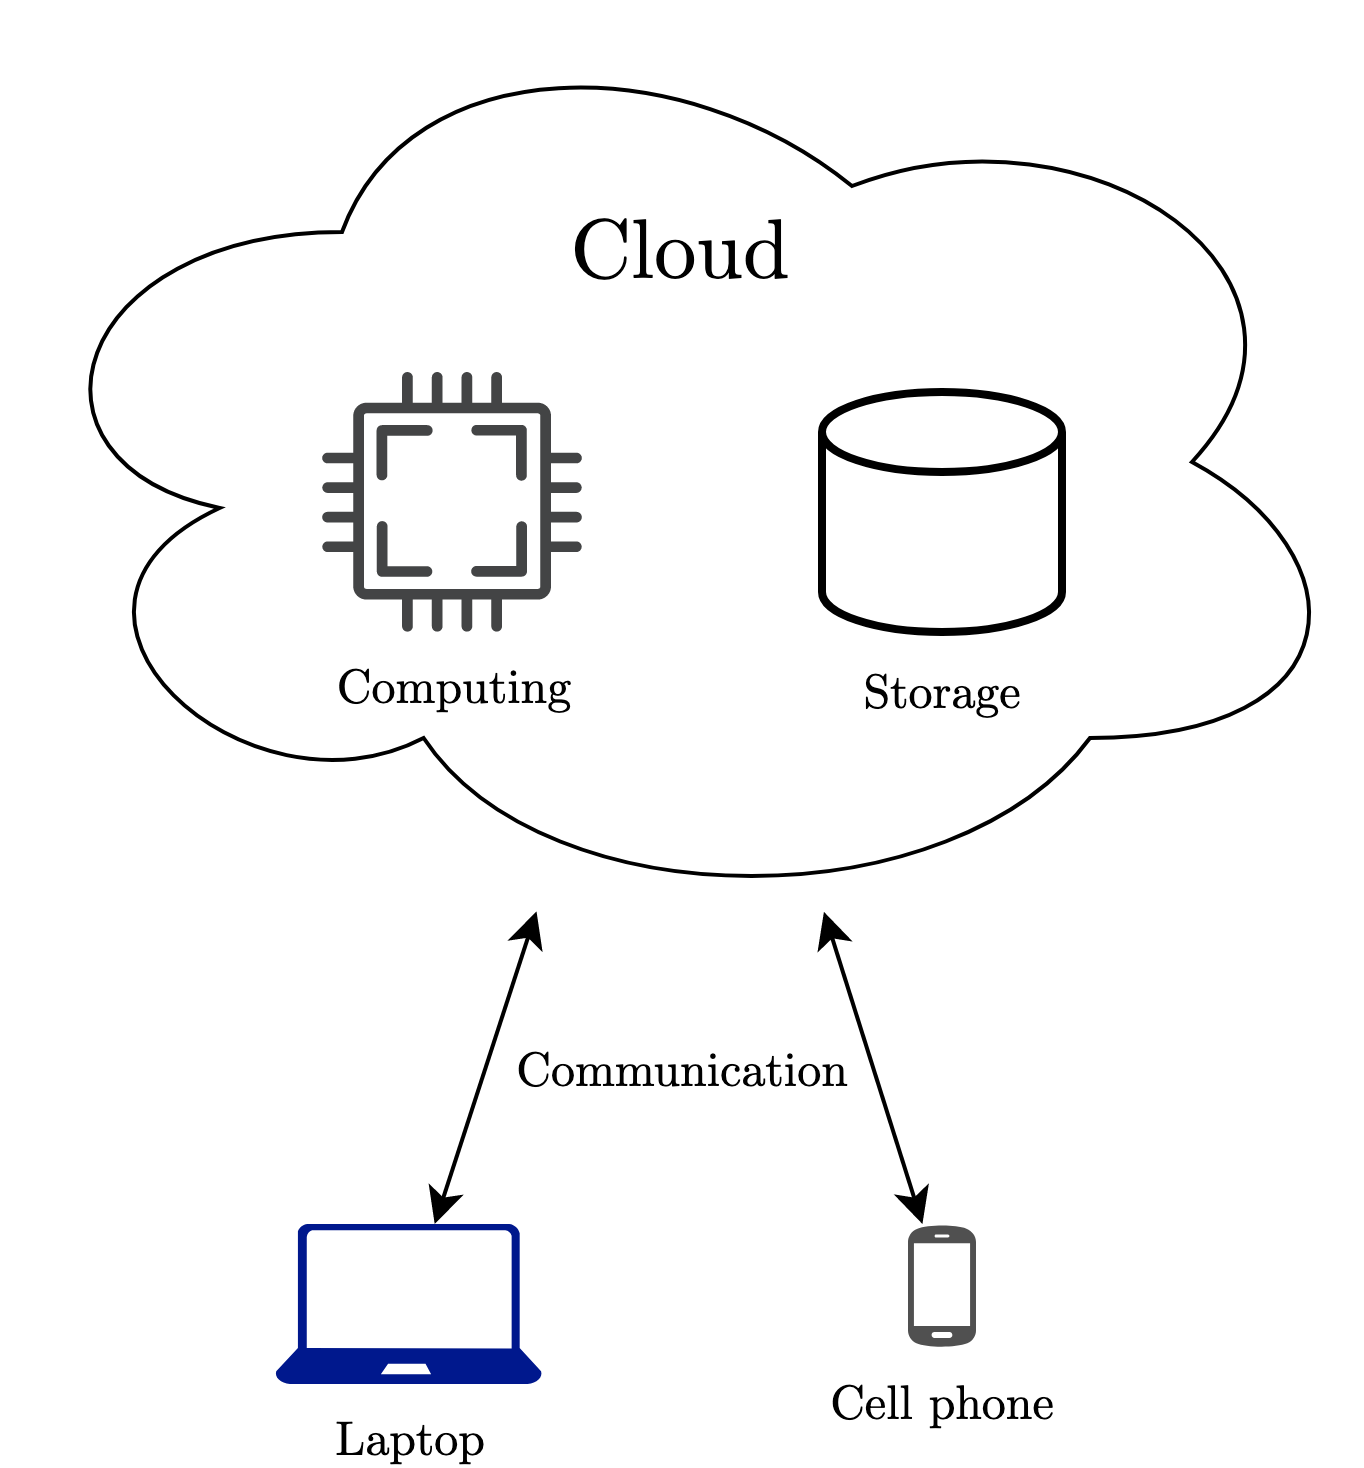
\includegraphics[scale=0.7]{chapters/background/figures/Simplified_cloud.png}
    \caption{A Simplified diagram of Cloud Computing}
    \label{fig:SimplifiedCloudDiagram}
\end{figure}

At a very high level, Cloud Computing is where you offload your work to the usually distant cloud. As shown on figure~\ref{fig:SimplifiedCloudDiagram}, a laptop or any other device can communicate with the cloud, and let the cloud provide storage and computation. The Cloud is a distributed system which is usually built as a Grid Computing system in a data centre. When working with the cloud, we typically have thin clients and thick clients. For traditional cloud computing the thin client is for example your laptop or cell phone, while the thick client is the server or servers in the distant data centre.

However, in today's society it has of course become much more advanced. You have an increasing number of cloud service providers that offer Infrastructure as a Service(IaaS), Platform as a Service(PaaS) and Software as a Service(SaaS), like Amazon Web Services(AWS), Digital Ocean, Alibaba Cloud, Microsoft Azure and Google Cloud Platform(GCP) just to name a few. The biggest of them all is AWS, which holds almost half of the market share\cite{noauthor_cloud_2019}. The Cloud market made 129 billion dollars in 2020 alone\cite{noauthor_cloud_nodate}.

Big firms will most likely benefit from building their own data centres. However most companies are not in the Fortune 500 with big wallets and millions of clients. Most firms, which have significantly less clients, can save a lot of money and time by outsourcing to cloud providers instead. It makes scaling easy and you can have infrastructure set up in just a few minutes, so you can focus on actually developing your service. You don't need to hire technicians to maintain the servers. If you have clients all over the world, you can choose to set up servers near them, instead of being limited to the office or headquarters. You can easily scale up by requesting stronger hardware, or you can easily scale out by replicating or starting more servers. In other words, it is just really convenient for most modern companies.

Even though the largest cloud providers have established themselves in many places, it still might not be close enough geographically to the client. In latency aware applications you need to minimize the physical distance between the client and the server. Therefore you can use local cloud providers, or firms like Akamai which specializes in having server as close, and as few as possible hops away from the end users.





% ----------------------------------------------





\section{Fog Computing}

Vaquero and Rodero-Merino\cite{vaquero_finding_2014}, defines fog computing like this: 
\say{Fog computing is a scenario where a huge number of heterogeneous (wireless and sometimes autonomous) ubiquitous and decentralised devices communicate and potentially cooperate among them and with the network to perform storage and processing tasks without the intervention of third parties. These tasks can be for supporting basic network functions or new services and applications that run in a sandboxed environment. Users leasing part of their devices to host these services get incentives for doing so.}

As in other fields, there is no de-facto definition and is debatable. Since Fog Computing is a relatively new concept, different definitions will be used depending on the field they are in.

Fog computing is an extension of the Cloud Computing paradigm. You have some nodes, like servers or desktops, that you offload the computation and storage to. The difference is that in Fog computing the fog nodes are located close in proximity to the user\cite{msftadmin_concept_2020}, as shown in figure~\ref{fig:FogDiagram}. The distant cloud has way more resources that the nodes in the fog layer, but since the fog nodes are closer, they are great at doing latency sensitive work. The Fog nodes is usually defined as being on the same LAN, but some argue that you can put them further away to, at least geographically speaking. 

An example is if an ISP has some Fog nodes at the base of cell towers. This will enable cell phones, or other SIM-card enabled devices, to offload storage and computation easily through the cell network. The introduction of 5G for the mainstream could benefit a lot from this. The latency for 5g will most likely be the same, but since the devices using it are so close to the 5G tower, it does not matter that much. The increased bandwidth of 5G is what will help a lot, as you can offload bigger workloads. We will discuss this in the Mobile Edge Computing chapter later. 

In Fog computing you would like as few jumps as possible to the node. A jump is when you move from one network node to another, for example from a cellphone to an Access Point. If the nodes are on the same LAN, the number of jumps are predictable and low in frequency, at least compared to the number of jumps to a distant data centre. 


For comparison, a Traceroute\cite{noauthor_traceroute68_nodate} from Oslo, Norway to a PlanetLab server in Rostock, Germany had at least 11 hops. With each hop adding latency because of processing, it’s easy to conclude that it is beneficial to keep hops at a minimum.

\begin{figure}[t]
    \centering
    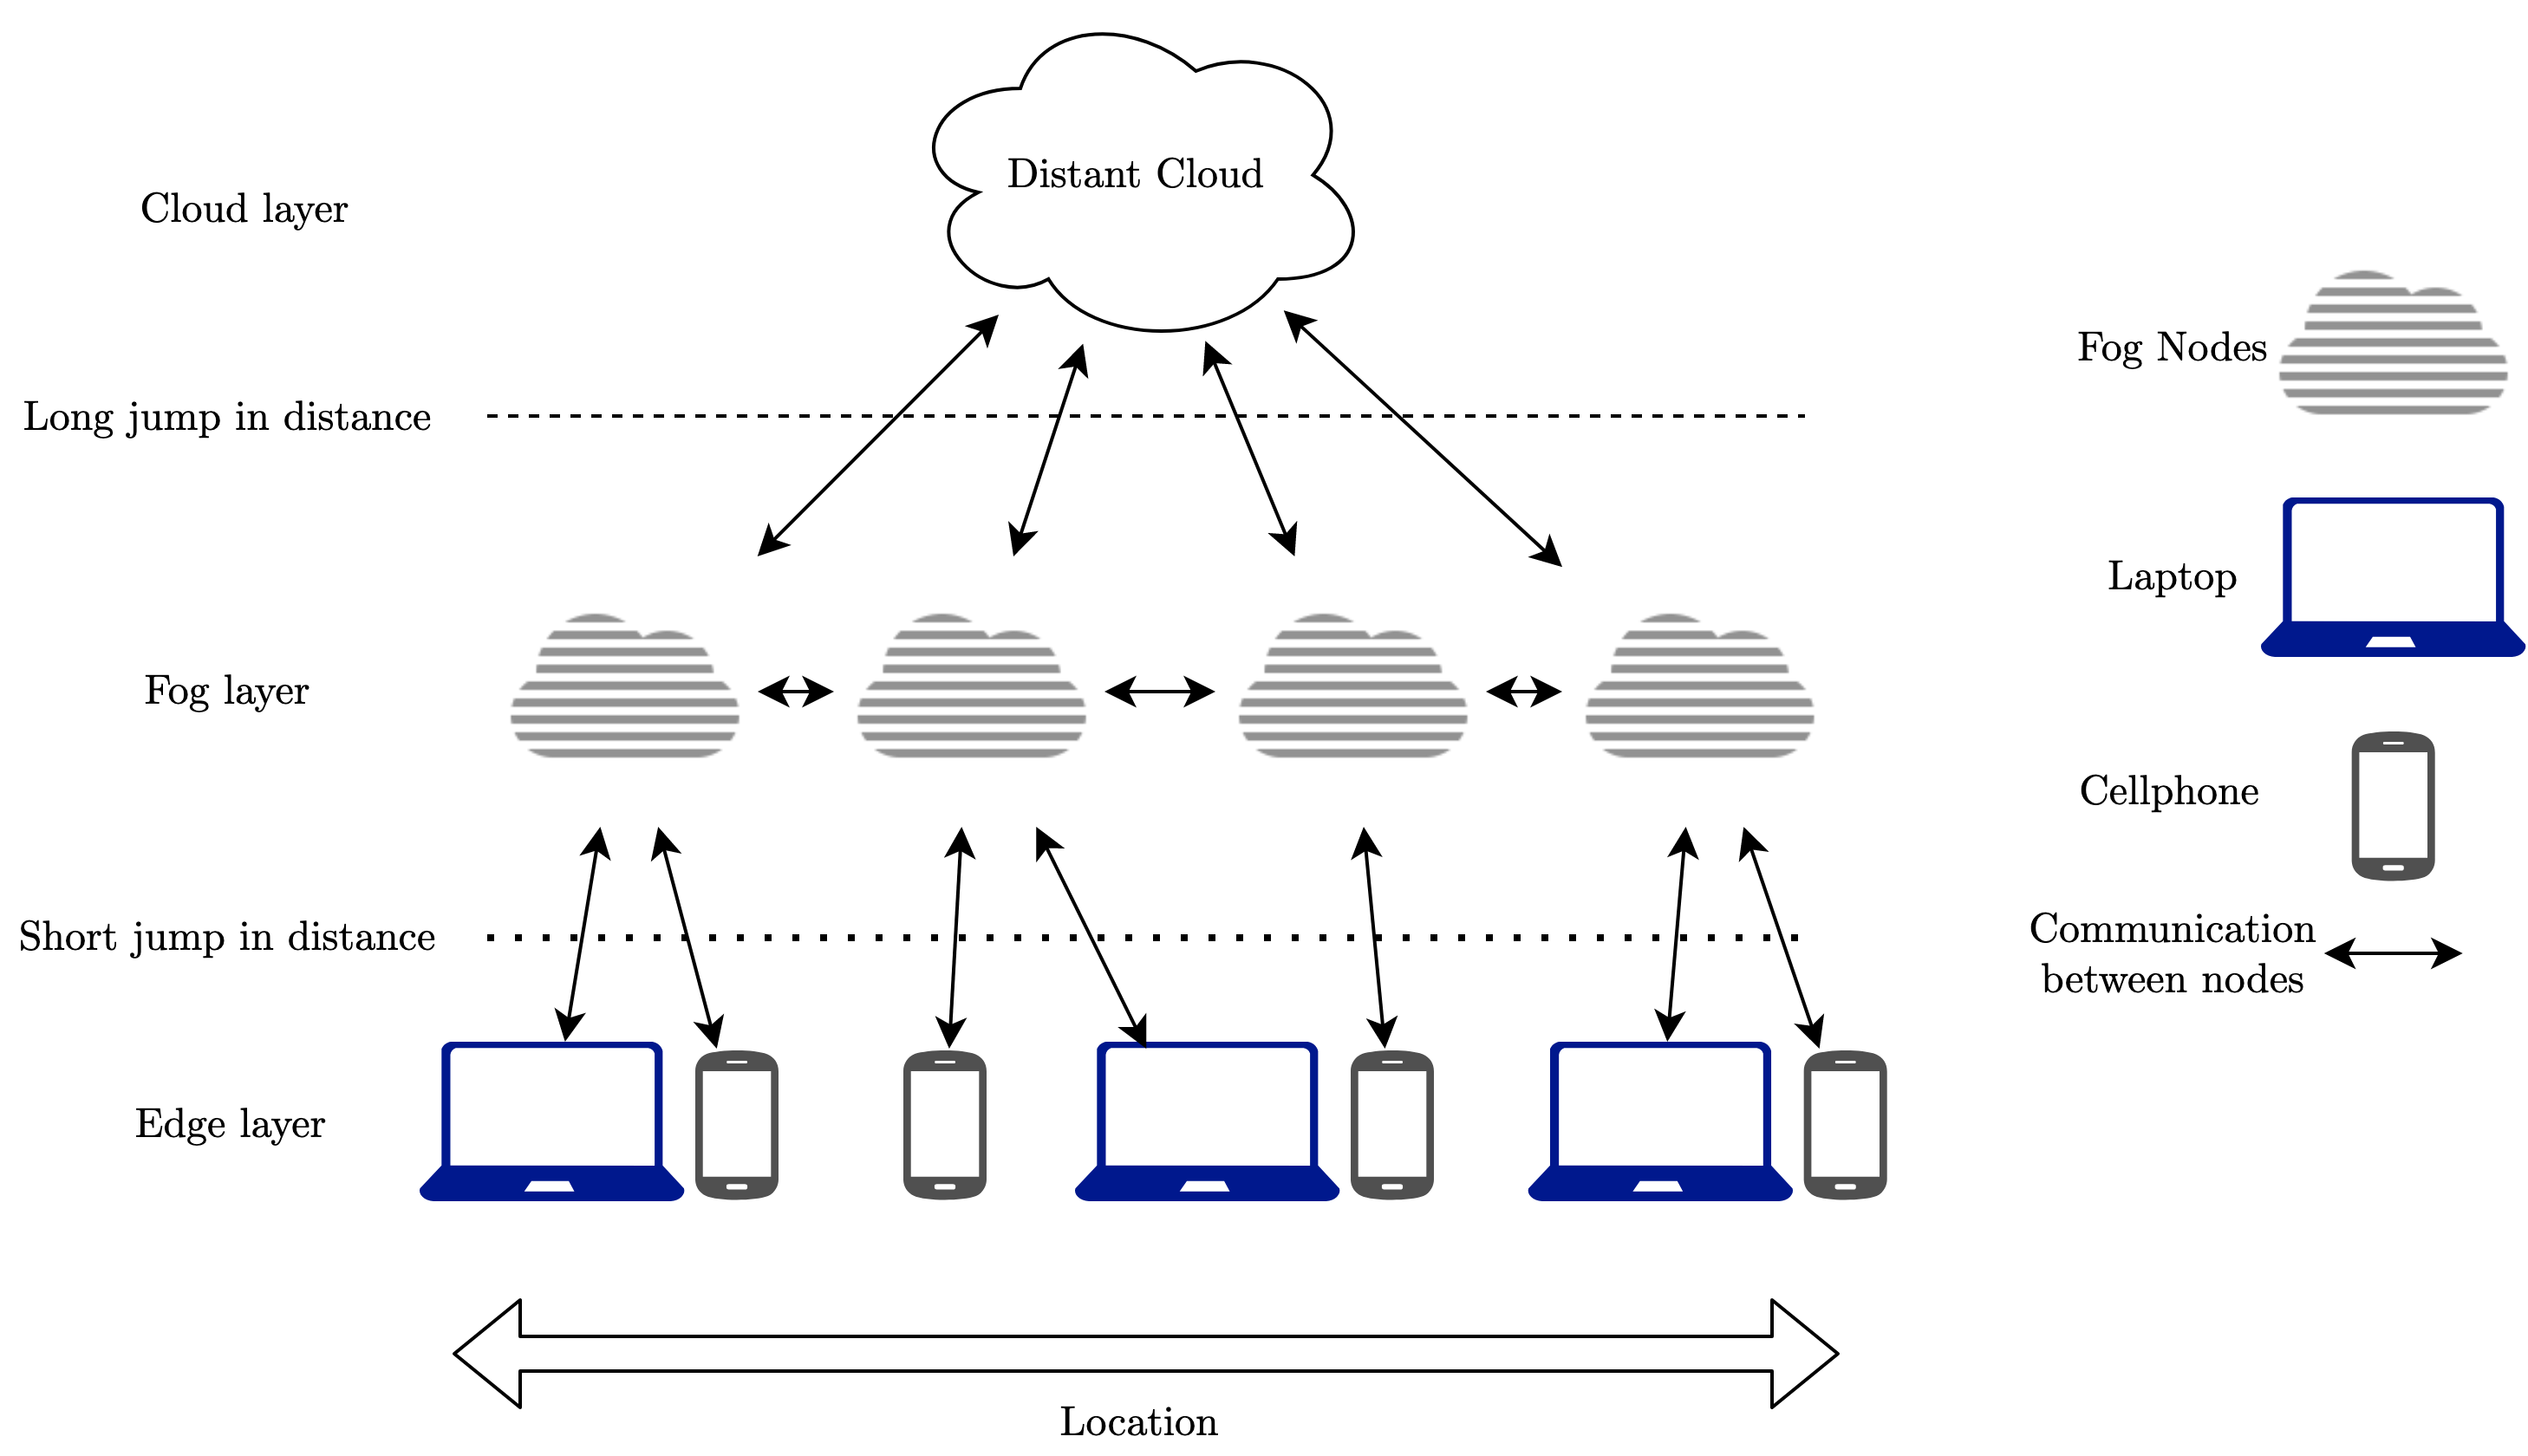
\includegraphics[scale=0.6]{chapters/background/figures/Fog.png}
    \caption{Diagram of Fog Computing}
    \label{fig:FogDiagram}
\end{figure}

\subsection{Cisco}
Cisco\cite{bonomi_fog_nodate} and Bonovi was the first to coin the term, and defines Fog Computing as \say{...a highly virtualized platform that provides compute, storage, and networking services between end devices and traditional Cloud Computing Data Centers, typically, but not exclusively located at the edge of network.}  The characteristics of Fog Computing is that it is located at the edge, has location awareness, low latency, easily geographically distributed, heterogeneity, support for mobility and some others. All these as a sum help with providing a service that is needed in some modern applications, for example Augmented Reality, and in general with IoT.

A Fog node is located at the edge in the sense that it is close to the end user or client. Because of this, the Fog node will have \textit{location awareness} and \textit{low latency}. Since they are not big servers, the Fog nodes are also easily \textit{geographically distributed}, in the sense that it should be easy to install and maintain. This also helps them be \textit{mobile}. Most likely the Fog nodes do not have the same hardware or software, which gives us the \textit{heterogeneity} characteristic. 

\subsection{A survey of Fog Computing} % TODO: REWRITE this
The goal of Fog Computing is to improve Quality of service(QoS) with computation and storage offloading. Yi, Li, and Li, in ‘A Survey of Fog Computing’\cite{yi_survey_2015} argues that QoS can be divided into four aspects: Connectivity, reliability, capacity and delay.

Connectivity in a fog network can be improved by network relaying, partitioning and clustering. They can be used to reduce cost, trim data and expand connectivity. Connectivity is of course important, because if you lose connection with the node, then you cannot offload work to it. 

Reliability is very difficult to provide in Fog computing. The methods used in traditional distributed systems like checkpointing and replication can be used. However since devices are more mobile, and nodes dynamic, this can be hard to implement. It also implies that Fog nodes are connected to each other, which is not given in all architectures. 

For capacity you need enough storage and good bandwidth. It does not matter how much storage you have, if it is slow to transfer it. To achieve good utilization of storage and bandwidth, it is important to analyse user patterns to know where data is most used. It’s difficult to know where to store data when it may need to be stored across several fog nodes. It is also hard to know when to send storage further to the distant cloud with bigger capacity at the cost of delay. 

Lastly, Fog focuses a lot on delay. It’s a good solution for “latency-sensitive” applications. There are several proposed solutions to minimize delay. We will discuss Cloudlets as a solution later.


% DETTE HØRER TIL I ARCHITECTURES
% \subsection{Fog architectures} %% move this to architectures?
% Naha et al.\cite{naha_fog_2018}, reviewed a couple of architectures that arguably falls under the Fog computing paradigm. We have focused on the ones that also fall under the Near-Far computing model, in that they have a Near node and a Far node. These architectures focus on offloading from an IoT device, to assist with computation, energy and storage. We will talk about IoT in a later chapter. 



% \subsubsection{Fog-Dew Computing (FD)}
% One drawback of Cloud computing is that you need to be always connected to the internet. 
% Fog-Dew Computing aims to provide IoT devices with cloud computing without being connected to the internet to reduce this issue. Depending on the application it might not need connection to the internet at all, while others can work temporarily offline but need to eventually connect to the internet. Fog-Dew Computing solves this by having an edge community server providing the needed cloud services. 




%----------------------------------








\section{Edge Computing}
Edge Computing is about utilizing processing power at the edge of the internet, instead of using data centers. The edge of the internet are the devices that are closest to the users and clients. It's very relevant for IoT, because IoT end devices generate a lot of data close to the users but far from the data centres. This makes it very inefficient to send the data all the way to the distant cloud. Since IoT often requires real time processing of data, it is better to move the processing to the edge, closer to the devices, to minimize the latency\cite{shi_edge_2016}.
A router, switch or Cloudlet are examples of an edge device. They can be utilized by the IoT devices to offload their computation to save time and energy.





%% ----------------------------------------------------------------------

\section{Ubiquitous computing and Internet Of Things}
%TODO
Internet of Things(IoT) is a system of ubiquitous devices that is connected to the Internet\cite{noauthor_what_nodate}. These devices are now everywhere in modern society. Things with a wide array of sensors are placed everywhere to solve problems or give us information. An example of this is smart watches. Smart watches has several to measure things like heart beat, geographical location, speed and so on. These devices give information to and takes information from the internet. These devices are often very small, have energy constraints because of small battery, and very limited storage. They there often offload computation and storage via its connection to the internet.





%% ----------------------------------------------------------------------

\section{The Near-Far Computing Model}
A definition of the Near-Far Computing Model will be discussed in a later chapter. However, a brief introduction is needed to understand what we are testing. The Near-Far Computing Model is a way to mitigate latency issues by having Near nodes and Far nodes. Near nodes are nodes that are geographically close by the client. This is beneficial, as the closer you are to the server, the lower the latency. Far nodes are  very strong servers that typically resides in distant data centers. The Near node is closer but not as powerful as the Far node. This lets us create a balance where the Near node can do low response time work, while the Far node provides more resources for heavier computations and storage that can afford the higher latency.



%%---------------------------------------------------------------------

\section{The slow speed of light}
The speed of light in a vacuum is 299,792 458 kilometers a second. This is the upper limit for how fast anything can travel. This also limits how fast electrons can move in cobber and how fast light can travel in fiber-optic cables. Signals in fiber-optic travels at about 2/3 of the speed of light. The speed of electrons in a copper wire is slight faster than fiber. However, clock speed of computers today are in the billions of times per second. If you have a CPU running at 5GHz, in other words 5 billion clock cycles a second, we can see that the computer has time to do quite a lot while waiting for packets. When a packet has traveled just 1 foot, which takes 1 nanosecond, the CPU has already done 5 clock cycles. If the packet is traveling to another country, we can easily see that the CPU can do quite a bit of work while waiting for that packet. Since the speed of light is not going to change, the only way to improve latency is to reduce the physical distance between the nodes.



%% ----------------------------------------------------------------------------


\section{Why high latency and low bandwidth hurts}


Humans will easily detect delay and jitter when using applications\cite{satyanarayanan_case_2009}. Delay is almost impossible to fight when using hardware that is physically a long distance away. Jitter is impossible to prevent when using WAN. As a consequence, user experience of applications using WAN might suffer. Applications where crispness and high response time is important is called \textit{latency-aware applications}. Niraj Tolia et al.\cite{tolia_quantifying_2006} showed that we can divide user perceived responsiveness into several bins:
\begin{center}
\begin{tabular}{ | p{3cm} | p{5cm} | } 
    \hline
    Response Time& Perceived Responsiveness  \\ 
    \hline
    < 150ms & Crisp  \\ 
    150ms - 1s & Noticeable to annoying \\ 
    1s - 2s & Annoying \\ 
    2s - 5s & Unacceptable \\ 
    > 5s & Unusable \\ 
    \hline
\end{tabular}
\end{center}
The response time of applications is the sum of the time taken for packets to be sent between nodes, plus the processing time. Latency is not the only factor for how slow data transferring can be. Bandwidth is also a really important factor\cite{cerqueira_interactive_2007}. Some applications require very high bandwidth, that is not necessarily available everywhere. When bandwidth is too low, the transferring time will take longer, which then affects the response time. 
For latency-aware applications, keeping the application crisp is important. There of course exists applications that needs way lower response time than 150ms. Some applications require response time down to a few milliseconds. An example of this is when surgeons use a remote controlled robot to perform surgery. In this situation responsiveness need real-time to ensure safety. 







% ------------------------------------------------------------------------  

\section{Emerald}\label{Emerald}
Emerald is a programming language created in the period of 1984-1986 by Eric B. Jul, Norm Hutchinson, Hank Levy and Andrew Black. It has several features that is important in distributed programming, like object mobility and type conformity. These features helps easing the development process of distributed systems. Emerald is an example that you can have object orientation in distributed systems that have similar performance as C++ in many aspects. This section will give an introduction to Emerald, and are mainly based on the Emerald Language Report\cite{hutchinson_emerald_nodate}

\subsection{Types and Conformity}
When programming distributed systems, each node has to agree on how to handle data. Emerald does this with types and conformity. Each node does not need to transfer or have a copy of the whole object. It only needs to know what that object has available, which can be described with types. When calling a remote node, we just need to get a copy of the object type to be able to know what to call, and what to send. Having strong compile-time typing ensures that we will always get the expected data, which reduces errors and failures.

Everything is an object in Emerald. Even types are just first-class objects. 
Emerald is a compile-time strongly typed language. This means that the compiler will check that all objects conforms to the types at compile time, except for a few cases. An object conforms to a type if
\begin{enumerate}
    \item All operations defined in the type is available in the object
    \item For each operation, there are the same number of parameters, and each parameter conforms to the corresponding parameters.
\end{enumerate}
There are more checks, but these two are the most important ones.
Here is an example:
\begin{lstlisting}[language=emerald]
type TypeA
    Integer multiplyByTwo[n: Integer]
end TypeA

const ObjectA <- class ObjectA
    operation multiplyByTwo[n: Integer]
                        <- [res: Integer]
        res <- n * 2
    end multiplyByTwo
end ObjectA
\end{lstlisting}
Here, the ObjectA conforms to TypeA because we have the \textit{multiplyByTwo} operation, the type of the parameter and the type of the return is the same as described in the type.

To enable generic types and polymorphism, Emerald lets you also check types during runtime with an operator: \verb|*>|. You can essentially read \verb|a *> b| as "\textit{a} conforms to \textit{b}". You also have \verb|view a as b| to help change the type of an object during runtime.




\subsubsection{Classes}
Emerald does not really have classes as everything is an object. We still have the concept of classes, and Emerald has the keyword \verb|class| to help us easily create it. Emerald will automatically create a type, a \textit{getSignature} operation, which returns the type, and finally a \textit{create} operation. These two objects are therefore semantically equivalent:
\begin{lstlisting}[language=emerald]
const A <- class A[x: Integer]
    export operation multiplyByTwo[n: Integer]
                        -> [res: Integer]
        res <- n * 2
    end multiplyByTwo
end A

const B <- object B
    const BType <- immutable typeobject BType
        operation multiplyByTwo[n: Integer]
                            -> [res: Integer]
    end BType
    export function getSignature -> [r: Signature]
        r <- BType
    end getSignature
    export operation create[x: Integer] -> [e: B]
        e <- immutable object aB
            export operation multiplyByTwo[n: Integer]
                        -> [res: Integer]
                res <- n * 2
            end multiplyByTwo
        end aB
    end create
end B
\end{lstlisting}
As you can see, using the \verb|class| keyword dramatically increases readability, gives us the consept of classes, and eases the development.

\subsection{Fields}\label{emerald:fields}
Emerald provides the keyword \verb|field| to automatically provide getters and setters.
\begin{lstlisting}[language=emerald]
const A <- class A
    field someVar : String <- ""
end A

const B <- class B
    var someVar: String <- ""
    
    export op getSomeVar -> [res: String]
        res <- someVar
    end getSomeVar
    
    export op setSomeVar[input: someVar]
        someVar <- input
    end setSomeVar
end B
\end{lstlisting}
In the above example, both class A and class B is equivalent. They will both have the operations \verb|getSomeVar| and \verb|setSomeVar| available.


\subsubsection{Immutability}
To ensure that objects does not change over time, we need immutability. This is important in distributed systems, as changing an object that was not meant to change can break how it is supposed to interpret data, as we can have nodes with different versions of the object. Since Emerald only copies over the type to other nodes, it is important that these types are not able to change(mutable). Therefore, all types should be mutable. Classes should be immutable if possible, to prevent confusion between nodes. The less mutable objects there are, the less errors and failure there can be.

\subsection{Object mobility}
One of the key features of Emerald is Object Mobility. It has the tools needed to easily move objects around in a distributed system. To move an object to a different node is as easy is this:
\begin{lstlisting}[language=emerald]
% x is created and resides on A
move x to B
% x now might reside on B
\end{lstlisting}
To visit all available nodes with your program is as easy as this\cite{noauthor_emerald_nodate}:
\begin{lstlisting}[language=emerald]
const Kilroy <- object Kilroy
  process
    const origin <-  locate self
    const up <- origin.getActiveNodes
    for e in up
      	const there <- e.getTheNode
      	move self to there
    end for
    move self to origin
  end process
end Kilroy
\end{lstlisting}
This short and simple compilable and runnable Emerald program will start a process, find all active nodes and then loop over and visit them, before going back to the original node.

The move keyword is more of a hint to the Emerald VM that the object should be moved over. In Emerald you can use \verb|fix| to tell the VM that it has to move the object, instead of it just being a hint. It has the same syntax as move:
\begin{lstlisting}[language=emerald]
% x is created and resides on A
fix x at B
% x now resides on B, and will not move until unfixed.
\end{lstlisting}
To move the object again, we now have to unfix it, which is done by using \verb|unfix|:
\begin{lstlisting}[language=emerald]
unfix x
\end{lstlisting}
The object can now be moved or fixed on a different location. To make this procedure easier we have the \verb|refix| keyword. It will unfix and then fix an object to a new location. In other words these are equivalent:
\begin{lstlisting}[language=emerald]
unfix x
fix x at C
\end{lstlisting}
and
\begin{lstlisting}[language=emerald]
refix x at C
\end{lstlisting}
Therefore we use refix almost everywhere when we are moving objects. 



\subsubsection{Attached}
When moving objects in Emerald, you are essentially just moving the pointer. This means that if you have an object with some inner variables, they will stay on the original node when the parent is moved. If it makes sense to move the related data with the object, which it usually does, we can use the \verb|attached| keyword.
As shown in figure~\ref{fig:emerald_attached_figure}, when using the Attached keyword, both the object and the attached objects will move over, when that parent object (x) is moved. If we do not move the related objects over, then there will be a tremendous performance impact because local invocations are many times faster than remote invocations. Here is an example of how you can use attached:
\begin{lstlisting}[language=emerald]
const x <- class x
    attached const y <- someObject.create
    attached const z <- someObject.create
end x
\end{lstlisting}
In the above code example, you will get an object similar to the one shown in Node A in figure~\ref{fig:emerald_attached_figure} before the move.

\begin{figure}[t]
    \centering
    \textbf{Not attached vs Attached}\par\medskip
    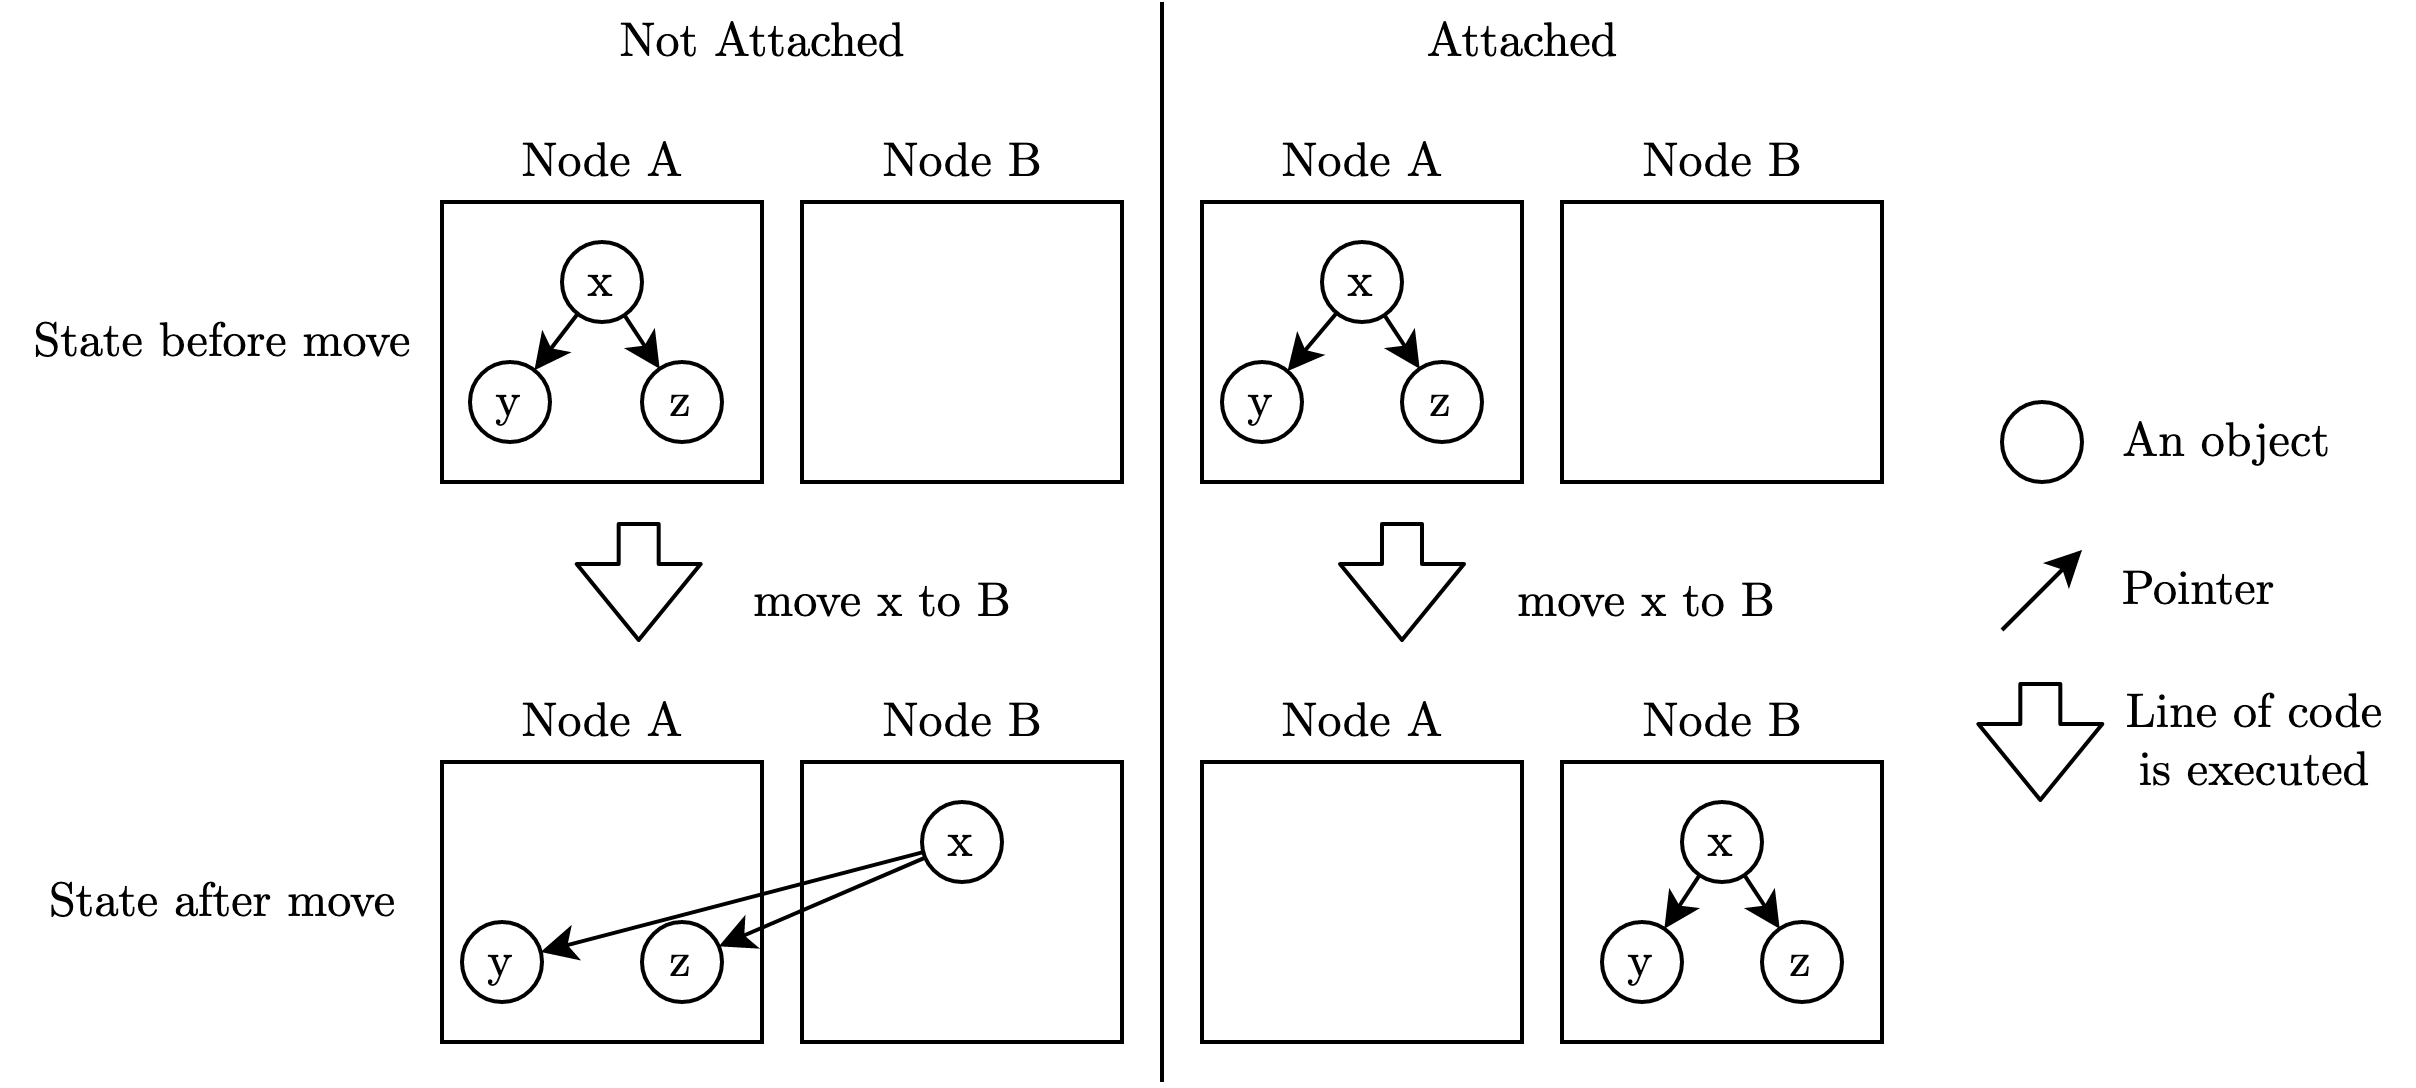
\includegraphics[scale=0.8]{chapters/background/figures/emerald_attached.png}
    \caption{Showing a move executed without and with attached objects}
    \label{fig:emerald_attached_figure}
\end{figure}

\subsubsection{Call-by-visit and call-by-move}
Call-by-visit and call-by-move are very similar concepts as attached. In Emerald you can use them to specify when you want to move the objects you send as parameters when invoking a function on a remote node. When using call-by-visit you move the parameters over, then move then back when finished with the function. When using call-by-move, you do the same, except the object stay on the remote node.

\subsubsection{How the Emerald VM finds the location of objects}\label{cascading_search}
Emerald has a system for keeping track of and finding objects. To get the location of an object you can use the \verb|locate| keyword. For example:
\begin{lstlisting}[language=emerald]
const x <- 3
move x to B
var locationOfX : Node <- locate x
% The variable "locationOfX" now holds 
%  the Node object that resides on B.
\end{lstlisting}
Emerald uses something called \textit{Cascading Search} to locate an object. To prevent having to broadcast each time an object moves, a node only keeps track of the last position it knows the object resides or resided on. If the last known position of X is on A, then we just ask the A if he can send it. If A has later moved X to node C, then it will just send the query to C. This is called a Forwarding Reference. It keeps track of last known location (from its own perspective) and also a counter. Each time an object moves, that counter is incremented on the receiving node. If node A moves object X to B, then the counter is 0 at A and 1 at B. That means that the higher the counter, the more recent the pointer is. The counter is essentially replacing a global clock, since having synchronized time is almost impossible in a distributed system. The algorithm also have ways of dealing with failing nodes and lost pointers, but we wont go any deeper into that. 


\subsection{Remote Procedure Call}
Emerald uses Remote Procedure Calls, which means that it will handle all remote invocations for you. Therefore, when programming, you can just invoke the object as if it were local. This ensures that programming with distributed objects is really easy, as you do not need to think about programming each remote invocation. Here is a comparison:
\begin{lstlisting}[language=emerald, numbers=left]
const A <- class A
    export function multiplyByTwo[i: Integer] 
                                -> [res: Integer]
        res <- i * 2
    end mulitplyByTwo
end A

const B <- object B
    initially
        const x <- A.create
        % x is now a local pointer to A
        const result1 <- x.multiplyByTwo[2]
        
        refix x at someOtherNode
        % x is now a remote pointer to A
        const result2 <- x.multiplyByTwo[2] 
    end initially
end B
\end{lstlisting}
On line 12 and 16, we do the same invocation, but the location of the invoked function is different.

If we try to invoke a function on a node that is not available, Emerald will raise 




\subsection{Failure and Unavailable}
When programming distributed systems we need to account for nodes going up or down. To help with this, Emerald has introduced \textbf{unavailable handlers}. Unavailable handlers can be put at the bottom of process blocks, functions and compound blocks. Within an unavailable handler, one can try to recover by trying again or by trying other nodes, for example.

\textbf{Failure Handlers} are invoked when a failure is raised by the program. An example of this is when invoking a nil object. The failure handler can be used to try to recover the program.

Below is an example of both failure and unavailable handlers:
\begin{lstlisting}[language=emerald, numbers=left]
const A <- class A
    export function divideTwoBy[i: Integer] 
                                -> [res: Integer]
        begin %compound statement
            res <- 2 / i
            failure
                % This will be executed if i is 0
            end failure
        end
    end mulitplyByTwo
end A

const B <- object B
    initially
        const x <- A.create
        % x is now a local pointer to A
        const result1 <- x.divideTwoBy[0]
        
        refix x at someOtherNode
        % x is now a remote pointer to A
        const result2 <- x.divideTwoBy[0]
        
        unavailable
            % this will be executed if someOtherNode
            %  is unavailable
        end unavailable
    end initially
end B
\end{lstlisting}






\subsection{Checkpoints and Recovery}
To help keeping nodes up, Emerald provides checkpoints and recovery blocks. At any point you can use the reserved \verb|checkpoint| keyword to create a checkpoint of an object. The checkpoint is just a saved state on the machine, so that the state is available on the disk instead of just RAM. If a node has restarted, then it will load the last checkpoint. When the program is recovering, the \verb|recovery| block is ran instead of the initially block. This is essential for creating more reliable distributed systems.



\subsection{Concurrency}
Emerald has support for processes, and they are really easy to set up. You use the process block like this:
\begin{lstlisting}[language=emerald]
const A <- class A
    process
        % do work here
    end process
end A
\end{lstlisting}

Emerald has also implemented monitors based on Hoare's monitors\cite{hoare_monitors_1974}. You can use the keywords \verb|monitor|, \verb|wait|, \verb|signal| and the \verb|Condition| type to easily have control over concurrency. Here is an example:
\begin{lstlisting}[language=emerald, numbers=left]
const A <- monitor class A
    const cond: Condition <- Condition.create
    export function multiplyByTwo[i: Integer] 
                                -> [res: Integer]
        wait cond % wait for your turn
        res <- i * 2
        signal cond % signal to _one_ other process
    end mulitplyByTwo
end A
\end{lstlisting}
In this example, line 6 will not be executed at the same time as other processes.







\subsection{Compiling and running}
You can compile Emerald with the Emerald Compiler\cite{noauthor_emeraldold-emerald_2019}, which, when installed, can be run in a terminal with \verb|ec|. When you have written you program you compile the files with \verb|ec| like this:
\begin{lstlisting}[language=Bash]
ec file1.m file2.m 
\end{lstlisting}
To then run the program, you use the \verb|emx| which will run the compiled program on the Emerald VM:
\begin{lstlisting}[language=Bash]
emx file1.x file2.x
\end{lstlisting}

To start a remote node, run this on the remote node:
\begin{lstlisting}[language=Bash]
emx -U -R
\end{lstlisting}
Then all the other additional nodes is started like this:
\begin{lstlisting}[language=Bash]
emx -U -R172.17.0.2
\end{lstlisting}
Here \textbf{172.17.0.2} is the IP address of the first node.
Finally, to run the program run this:
\begin{lstlisting}[language=Bash]
emx -U -R172.17.0.2 file1.x file2.x
\end{lstlisting}
All the other nodes are now accessible, and can have objects moved to them.



%% ---------------------------------------------------------

\section{Docker}\label{background:docker}
Docker is a tool for running programs on the same architecture everywhere, without spinning up a whole virtual machine. It is built around the concept of \textit{containers}. Containers are small packages of software, that run on the Docker Engine. The Docker Engine is the the middleware between the containers and the operating system. This lets us run something locally and be able to expect the same behavior on other machines. Therefore, no matter where you run the application, it will always be the same environment from the perspective of the program. 

Because a Docker does not spin up a whole virtual machine, but rather share some resources with between the containers \cite{dockercom_what_nodate}, it is more efficient. The container is essentially a sandbox, that runs on top of the OS. Each of the applications are therefore isolated, even though they have some shared resources.

To run Emerald we use a stripped debian image with i386 architecture, made by Oleks Shturmov\cite{oleks_oleksdocker-in5570v21_2021}.
In the referenced github repository, Oleks provides a makefile to easily set up Emerald.



%%------------------------------------------------------
\section{PlanetLab}
PlanetLab is virtual organization consisting of many nodes spread out over the world. If an institution, like an university, wants to use PlanetLab, then they have to provide a PlanetLab server themselves. In other word, the institution get sent a server, which they have to install and maintain to keep using PlanetLab. This ensures that you get a wide network that spans all over the world. At it's peak, it had 1353 nodes spread across the earth\cite{noauthor_planetlab_nodate}. It is used as a wide-area network to do research on distributed systems. To get access you request for a DIKU, which is a collection of servers that you can log into. The login username for the servers, is then the name of the DIKU.

Each of the nodes run some from an operating system. We can connect to them with Secure Shell(SSH). Each node we use in this thesis will have Docker available. To run Emerald on a PlanetLab server, transfer the Emerald source code or executable and the makefile for running Emerald, over to the server with scp. For example, transfer the folder you are currently in to the home folder on the remote server:
\begin{lstlisting}[language=Bash]
scp -r . "planetlab-1.ida.liu.se":"~/"
\end{lstlisting}
Then ssh into the server: 
\begin{lstlisting}[language=Bash]
ssh -i ~/.ssh/planetlab \
    -l diku_name \
    "planetlab-1.ida.liu.se"
\end{lstlisting}
Here we provide a PlanetLab ssh key and the login name, which is the name of the DIKU, and a server URL.

When logged in on the server, we run the makefile with \verb|make| to start the shell within the Docker container. Then you can either run the executable, or compile the code as described in the Emerald section \ref{Emerald}.



\section{Summary}
In this chapter we have made a theoretical foundation to help understanding this thesis. We have described what a distributed system is, what it consists of, and some key features about it. We have given a short introduction to Edge, Fog and Cloud computing. We have also made a short description of Near-Far computing, explained what speed of light have to do with latency, and showed how the Emerald eco-system works. Finally we have given a description of the environment the experiments will be conducted on, with Docker and PlanetLab.

%% TODO:

%% LAG FIGURES TIL DISTRIBUTED SYSTEMS

% Snakk om Why latency hurts? Snakk om hvorfor vi offloader?

% iot

%NFV og SDN?